\section{Die Simulation}
\begin{figure}
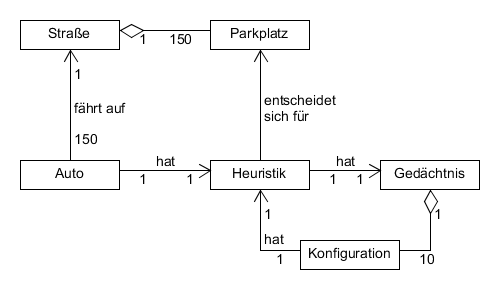
\includegraphics[width=0.5\textwidth]{uml/simOverview.png}
\caption{Strukturelle Übersicht der Simulation}\label{fig_simOver}
\end{figure}
Um die Konfigurationen für die Heuristiken zu lernen wird die Parkplatzsuche simuliert. Da in dieser Arbeit mehrere Fragen beantwortet werden sollen, sind auch mehrere Simulationen mit unterschiedlichen Randbedingungen notwendig. Der Grundlegende Aufbau jeder Simulation ist jedoch gleich und in Abbildung \ref{fig_simOver} dargestellt. Die Simulation ist objekt-orientiert aufgebaut. Die Straße verwaltet dabei sowohl die Autos und die Parkplätze als auch die diskreten zeitschritte der Simulation. Autos fahren zu einem zufälligen Zeitpunkt in die Straße ein und erreichen in jedem Zeitschritt, im Folgenden \emph{tick} genannt, einen Parkplatz. Dieser wird von der Heuristik des Autos, die man als den Fahrer des Autos interpretieren kann, evaluiert diesen Parkplatz, sofern er noch nicht belegt ist. Entscheidet sich die Heuristik für den Parkplatz parkt auch das Auto für eine bestimmte Zeit auf ihm. Das Ausparken wird nur durch die Freigabe des Parkplatzes nach der Parkzeit des Autos modelliert. Um zu garantieren, dass immer Parkplätze gefunden werden, werden in den Simulationen genausoviele Autos eingesetzt wie Parkplätze vorhanden sind. Die genaue Implementierung wird im Anhang erläutert.

\subsection{Wahl der Parameter}
Jede der durchgeführten Simulationen hat eine Dauer von $10^7$ Ticks und eine Straße mit $150$ Parkplätzen. Die Topologie der Straße ist die von Hutchinson et al. \textbf{cite}
\begin{figure}
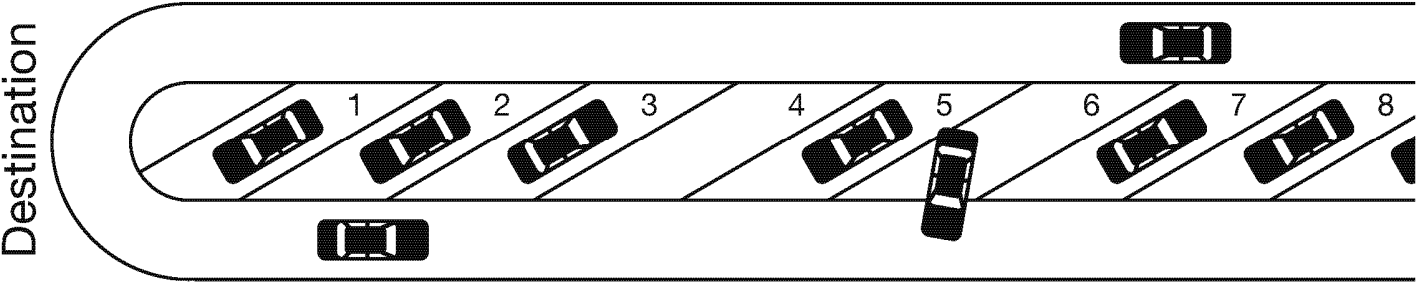
\includegraphics[width=\textwidth]{pics/street.png}
\caption{textbf{cite}, Topologie der Straße}
\end{figure}




\subsection{Unterschiede zu Hutchinson et al}

